
%{{第三十回}}{第三十回}}

\chapter{宝钗借扇机带双敲\hspace{.5em}龄官划蔷痴及局外}

{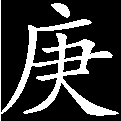
\includegraphics[width=3mm]{../Images/00004}借扇敲双玉,是写宝钗金蝉脱壳。}

{银钗画``蔷''字,是{[}写{]}痴女梦中说梦。}

{脚踢袭人,是断无是理,竟有是事。}

话说林黛玉与宝玉角口后,也自后悔,但又无去就他之理,因此日夜闷闷,如有所失。紫鹃度其意,乃劝道:``若论前日之事,竟是姑娘太浮躁了些。别人不知宝玉那脾气,难道咱们也不知道的?为那玉也不是闹了一遭两遭了。''黛玉啐道:``你倒来替人派我的不是。我怎么浮躁了?''紫鹃笑道:``好好的,为什么又剪了那穗子?岂不是宝玉只有三分不是,姑娘倒有七分不是。我看他素日在姑娘身上就好,皆因姑娘小性儿,常要歪派他,才这么样。''

林黛玉正欲答话,只听院外叫门。紫鹃听了一听,笑道:``这是宝玉的声音,想必是来赔不是来了。''林黛玉听了道:``不许开门!''紫鹃道:``姑娘又不是了。这么热天毒日头地下,晒坏了他如何使得呢!''口里说着,便出去开门,果然是宝玉。一面让他进来,一面笑道:``我只当是宝二爷再不上我们这门了,谁知这会子又来了。''宝玉笑道:``你们把极小的事倒说大了。好好的为什么不来?我便死了,魂也要一日来一百遭。妹妹可大好了?''紫鹃道:``身上病好了,只是心里气不大好。''宝玉笑道:``我晓得有什么气。''一面说着,一面进来,只见林黛玉又在床上哭。

那林黛玉本不曾哭,听见宝玉来,由不得伤了心,止不住滚下泪来。宝玉笑着走近床来,道:``妹妹身上可大好了?''林黛玉只顾拭泪,并不答应。宝玉因便挨在床沿上坐了,一面笑道:``我知道妹妹不恼我。但只是我不来,叫旁人看着,倒像是咱们又拌了嘴的似的。若等他们来劝咱们,那时节岂不咱们倒觉生分了?不如这会子,你要打要骂,凭着你怎么样,千万别不理我。''说着,又把``好妹妹''叫了几万声。林黛玉心里原是再不理宝玉的,这会子见宝玉说别叫人知道他们拌了嘴就生分了似的这一句话,又可见得比人原亲近,因又撑不住哭道:``你也不用哄我。从今以后,我也不敢亲近二爷,二爷也全当我去了。''宝玉听了笑道:``你往那去呢?''林黛玉道:``我回家去。''宝玉笑道:``我跟了你去。''林黛玉道:``我死了。''宝玉道:``你死了,我做和尚!''林黛玉一闻此言,登时将脸放下来,问道:``想是你要死了,胡说的是什么!你家倒有几个亲姐姐亲妹妹呢,明儿都死了,你几个身子去作和尚?明儿我倒把这话告诉别人去评评。''

宝玉自知这话说的造次了,后悔不来,登时脸上红胀起来,低着头不敢则一声。幸而屋里没人。林黛玉直瞪瞪的瞅了他半天,气的一声儿也说不出来。见宝玉憋的脸上紫胀,便咬着牙用指头狠命的在他额颅上戳了一下,``哼''了一声,咬牙说道:``你这------''刚说了两个字,便又叹了一口气,仍拿起手帕子来擦眼泪。宝玉心里原有无限的心事,又兼说错了话,正自后悔;又见黛玉戳他一下,要说又说不出来,自叹自泣,因此自己也有所感,不觉滚下泪来。要用帕子揩拭,不想又忘了带来,便用衫袖去擦。林黛玉虽然哭着,却一眼看见了,见他穿着簇新藕合纱衫,竟去拭泪,便一面自己拭着泪,一面回身将枕边搭的一方绡帕子拿起来,向宝玉怀里一摔,一语不发,仍掩面自泣。宝玉见他摔了帕子来,忙接住拭了泪,{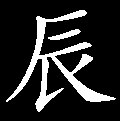
\includegraphics[width=3mm]{../Images/00009}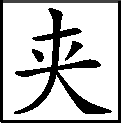
\includegraphics[width=3mm]{../Images/00012}\footnotesize \kaishu 写尽宝、黛无限心曲,假使圣叹见之,正不知批出多少妙处。}又挨近前些,伸手拉了林黛玉一只手,笑道:``我的五脏都碎了,你还只是哭。走罢,我同你往老太太跟前去。''林黛玉将手一摔道:``谁同你拉拉扯扯的。一天大似一天的,还这么涎皮赖脸的,连个道理也不知道。''

一句没说完,只听喊道:``好了!''宝林二人不防,都唬了一跳,回头看时,只见凤姐儿跳了进来,笑道:``老太太在那里抱怨天抱怨地,只叫我来瞧瞧你们好了没有。我说不用瞧,过不了三天,他们自己就好了。老太太骂我,说我懒。我来了,果然应了我的话了。也没见你们两个人有些什么可拌的,三日好了,两日恼了,越大越成了孩子了!有这会子拉着手哭的,昨儿为什么又成了乌眼鸡呢!还不跟我走,到老太太跟前,叫老人家也放些心。''说着拉了林黛玉就走。林黛玉回头叫丫头们,一个也没有。凤姐道:``又叫他们作什么,有我伏侍你呢。''一面说,一面拉了就走。宝玉在后面跟着出了园门。到了贾母跟前,凤姐笑道:``我说他们不用人费心,自己就会好的。老祖宗不信,一定叫我去说合。我及至到那里要说合,谁知两个人倒在一处对赔不是了。对哭对诉,倒像`黄鹰抓住了鹞子的脚',两个都扣了环了,那里还要人去说合。''说的满屋里都笑起来。

此时宝钗正在这里。那林黛玉只一言不发,挨着贾母坐下。宝玉没甚说的,便向宝钗笑道:``大哥哥好日子,偏生我又不好了,没别的礼送,连个头也不得磕去。大哥哥不知我病,倒像我懒,推故不去的。倘或明儿闲了,姐姐替我分辩分辩。''宝钗笑道:``这也多事。你便要去也不敢惊动,何况身上不好,弟兄们日日一处,要存这个心倒生分了。''宝玉又笑道:``姐姐知道体谅我就好了。''又道:``姐姐怎么不看戏去?''宝钗道:``我怕热,看了两出,热的很。要走,客又不散。我少不得推身上不好,就来了。''宝玉听说,自己由不得脸上没意思,只得又搭讪笑道:``怪不得他们拿姐姐比杨妃,原来也体丰怯热。''宝钗听说,不由的大怒,待要怎样,又不好怎样。回思了一回,脸红起来,便冷笑了两声,说道:``我倒像杨妃,只是没一个好哥哥好兄弟可以作得杨国忠的!''二人正说着,可巧小丫头靛儿因不见了扇子,和宝钗笑道:``必是宝姑娘藏了我的。好姑娘,赏我罢。''宝钗指他道:``你要仔细!我和你顽过,你再疑我。和你素日嘻皮笑脸的那些姑娘们跟前,你该问他们去。''说的个靛儿跑了。宝玉自知又把话说造次了,当着许多人,更比才在林黛玉跟前更不好意思,便急回身又同别人搭讪去了。

林黛玉听见宝玉奚落宝钗,心中着实得意,才要搭言也趁势儿取个笑,不想靛儿因找扇子,宝钗又发了两句话,他便改口笑道:``宝姐姐,你听了两出什么戏?''宝钗因见林黛玉面上有得意之态,一定是听了宝玉方才奚落之言,遂了他的心愿,忽又见问他这话,便笑道:``我看的是李逵骂了宋江,后来又赔不是。''宝玉便笑道:``姐姐通今博古,色色都知道,怎么连这一出戏的名字也不知道,就说了这么一串子。这叫《负荆请罪》。''宝钗笑道:``原来这叫作《负荆请罪》!你们通今博古,才知道`负荆请罪',我不知道什么是`负荆请罪'!''一句话还未说完,宝玉林黛玉二人心里有病,听了这话早把脸羞红了。凤姐于这些上虽不通达,但只见他三人形景,便知其意,便也笑着问人道:``你们大暑天,谁还吃生姜呢?''众人不解其意,便说道:``没有吃生姜。''凤姐故意用手摸着腮,诧异道:``既没人吃生姜,怎么这么辣辣的?''宝玉黛玉二人听见这话,越发不好过了。宝钗再要说话,见宝玉十分讨愧,形景改变,也就不好再说,只得一笑收住。别人总未解得他四个人的言语,因此付之流水。

一时宝钗凤姐去了,林黛玉笑向宝玉道:``你也试着比我利害的人了。谁都像我心拙口笨的,由着人说呢。''宝玉正因宝钗多了心,自己没趣,又见林黛玉来问着他,越发没好气起来。待要说两句,又恐林黛玉多心,说不得忍着气,无精打采一直出来。

谁知目今盛暑之时,又当早饭已过,各处主仆人等多半都因日长神倦之时,宝玉背着手,到一处,一处鸦雀无闻。从贾母这里出来,往西走过了穿堂,便是凤姐的院落。到他们院门前,只见院门掩着。知道凤姐素日的规矩,每到天热,午间要歇一个时辰的,进去不便,遂进角门,来到王夫人上房内。只见几个丫头子手里拿着针线,却打盹儿呢。王夫人在里间凉榻上睡着,金钏儿坐在旁边捶腿,也乜斜着眼乱恍。

宝玉轻轻的走到跟前,把他耳上带的坠子一滴\href{../Text/part0034_split_000.html\#lnkback_1_a}{\textsuperscript{①}},金钏儿睁开眼,见是宝玉。宝玉悄悄的笑道:``就困的这么着?''金钏抿嘴一笑,摆手令他出去,仍合上眼。宝玉见了他,就有些恋恋不舍的,悄悄的探头瞧瞧王夫人合着眼,便自己向身边荷包里带的香雪润津丹掏了出来,便向金钏儿口里一送。金钏儿并不睁眼,只管噙了。宝玉上来便拉着手,悄悄的笑道:``我明日和太太讨你,咱们在一处罢。''金钏儿不答。宝玉又道:``不然,等太太醒了我就讨。''金钏儿睁开眼,将宝玉一推,笑道:``你忙什么!`金簪子掉在井里头,有你的只是有你的',连这句话语难道也不明白?我倒告诉你个巧宗儿,你往东小院子里拿环哥儿同彩云去。''宝玉笑道:``凭他怎么去罢,我只守着你。''只见王夫人翻身起来,照金钏儿脸上就打了个嘴巴子,指着骂道:``下作小娼妇,好好的爷们,都叫你教坏了。''宝玉见王夫人起来,早一溜烟去了。

这里金钏儿半边脸火热,一声不敢言语。登时众丫头听见王夫人醒了,都忙进来。王夫人便叫玉钏儿:``把你妈叫来,带出你姐姐去。''金钏儿听说,忙跪下哭道:``我再不敢了。太太要打骂,只管发落,别叫我出去就是天恩了。我跟了太太十来年,这会子撵出去,我还见人不见人呢!''王夫人固然是个宽仁慈厚的人,从来不曾打过丫头们一下,今忽见金钏儿行此无耻之事,此乃平生最恨者,故气忿不过,打了一下,骂了几句。虽金钏儿苦求,亦不肯收留,到底唤了金钏儿之母白老媳妇来领了下去。那金钏儿含羞忍辱的出去,不在话下。

且说宝玉见王夫人醒来,自己没趣,忙进大观园来。只见赤日当空,树阴合地,满耳蝉声,静无人语。刚到了蔷薇花架,只听有人哽噎之声。宝玉心中疑惑,便站住细听,果然架下那边有人。如今五月之际,那蔷薇正是花叶茂盛之际,宝玉便悄悄的隔着篱笆洞儿一看,只见一个女孩子蹲在花下,手里拿着根绾头的簪子在地下抠土,一面悄悄的流泪。宝玉心中想道:``难道这也是个痴丫头,又像颦儿来葬花不成?''因又自叹道:``若真也葬花,可谓`东施效颦',不但不为新特,且更可厌了。''想毕,便要叫那女子,说:``你不用跟着那林姑娘学了。''话未出口,幸而再看时,这女孩子面生,不是个侍儿,倒像是那十二个学戏的女孩子之内的,却辨不出他是生旦净丑那一个角色来。宝玉忙把舌头一伸,将口掩住,自己想道:``幸而不曾造次。上两次皆因造次了,颦儿也生气,宝儿也多心,如今再得罪了他们,越发没意思了。''

一面想,一面又恨认不得这个是谁。再留神细看,只见这女孩子眉蹙春山,眼颦秋水,面薄腰纤,袅袅婷婷,大有林黛玉之态。宝玉早又不忍弃他而去,只管痴看。只见他虽然用金簪划地,并不是掘土埋花,竟是向土上画字。宝玉用眼随着簪子的起落,一直一画一点一勾的看了去,数一数,十八笔。自己又在手心里用指头按着他方才下笔的规矩写了,猜是个什么字。写成一想,原来就是个蔷薇花的``蔷''字。宝玉想道:``必定是他也要作诗填词。这会子见了这花,因有所感,或者偶成了两句,一时兴至恐忘,在地下画着推敲,也未可知。且看他底下再写什么。''一面想,一面又看,只见那女孩子还在那里画呢,画来画去,还是个``蔷''字。再看,还是个``蔷''字。里面的原是早已痴了,画完一个又画一个,已经画了有几十个``蔷''。外面的不觉也看痴了,两个眼睛珠儿只管随着簪子动,心里却想:``这女孩子一定有什么话说不出来的大心事,才这样个形景。外面既是这个形景,心里不知怎么熬煎。看他的模样儿这般单薄,心里那里还搁的住熬煎。可恨我不能替你分些过来。''

伏中阴晴不定,扇云可致雨,忽一阵凉风过了,唰唰的落下一阵雨来。宝玉看着那女子头上滴下水来,纱衣裳登时湿了。宝玉想道:``这时下雨。他这个身子,如何禁得骤雨一激!''因此禁不住便说道:``不用写了。你看下大雨,身上都湿了。''那女孩子听说倒唬了一跳,抬头一看,只见花外一个人叫他不要写了,下大雨了。一则宝玉脸面俊秀;二则花叶繁茂,上下俱被枝叶隐住,刚露着半边脸,那女孩子只当是个丫头,再不想是宝玉,因笑道:``多谢姐姐提醒了我。难道姐姐在外头有什么遮雨的?''一句提醒了宝玉,``嗳哟''了一声,才觉得浑身冰凉。低头一看,自己身上也都湿了。说声``不好'',只得一气跑回怡红院去了,心里却还记挂着那女孩子没处避雨。

原来明日是端阳节,那文官等十二个女子都放了学,进园来各处顽耍。可巧小生宝官、正旦玉官两个女孩子,正在怡红院和袭人顽笑,被大雨阻住。大家把沟堵了,水积在院内,把些绿头鸭、花鸂鶒、彩鸳鸯,捉的捉,赶的赶,缝了翅膀,放在院内顽耍,将院门关了。袭人等都在游廊上嘻笑。

宝玉见关着门,便以手扣门,里面诸人只顾笑,那里听见。叫了半日,拍的门山响,里面方听见了,估谅着宝玉这会子再不回来的。袭人笑道:``谁这会子叫门,没人开去。''宝玉道:``是我。''麝月道:``是宝姑娘的声音。''晴雯道:``胡说!宝姑娘这会子做什么来。''袭人道:``让我隔着门缝儿瞧瞧,可开就开,要不可开,叫他淋着去。''说着,便顺着游廊到门前,往外一瞧,只见宝玉淋的雨打鸡一般。袭人见了又是着忙又是可笑,忙开了门,笑的弯着腰拍手道:``这么大雨地里跑什么?那里知道爷回来了。''

宝玉一肚子没好气,满心里要把开门的踢几脚,及开了门,并不看真是谁,还只当是那些小丫头子们,便抬腿踢在肋上。袭人``嗳哟''了一声。宝玉还骂道:``下流东西们!我素日担待你们得了意,一点儿也不怕,越发拿我取笑儿了。''口里说着,一低头见是袭人哭了,方知踢错了,忙笑道:``嗳哟,是你来了!踢在那里了?''袭人从来不曾受过大话的,今儿忽见宝玉生气踢他一下,又当着许多人,又是羞,又是气,又是疼,真一时置身无地。待要怎么样,料着宝玉未必是安心踢他,少不得忍着说道:``没有踢着。还不换衣裳去。''

宝玉一面进房来解衣,一面笑道:``我长了这么大,今日是头一遭儿生气打人,不想就偏遇见了你!''袭人一面忍痛换衣裳,一面笑道:``我是个起头儿的人,不论事大事小事好事歹,自然也该从我起。但只是别说打了我,明儿顺了手也打起别人来。''宝玉道:``我才也不是安心。''袭人道:``谁说你是安心了!素日开门关门,都是那起小丫头子们的事。他们是憨皮惯了的,早已恨的人牙痒痒,他们也没个怕惧儿。你当是他们,踢一下子,唬唬他们也好些。才刚是我淘气,不叫开门的。''

说着,那雨已住了,宝官、玉官也早去了。袭人只觉肋下疼的心里发闹,晚饭也不曾好生吃。至晚间洗澡时脱了衣服,只见肋上青了碗大一块,自己倒唬了一跳,又不好声张。一时睡下,梦中作痛,由不得``嗳哟''之声从睡中哼出。宝玉虽说不是安心,因见袭人懒懒的,也睡不安稳。忽夜间听得``嗳哟'',便知踢重了,自己下床悄悄的秉灯来照。刚到床前,只见袭人嗽了两声,吐出一口痰来,``嗳哟''一声,睁开眼见了宝玉,倒唬了一跳道:``作什么?''宝玉道:``你梦里`嗳哟',必定踢重了。我瞧瞧。''袭人道:``我头上发晕,嗓子里又腥又甜,你倒照一照地下罢。''宝玉听说,果然持灯向地下一照,只见一口鲜血在地。宝玉慌了,只说:``了不得了!''袭人见了,也就心冷了半截。要知端的,且听下回分解。

{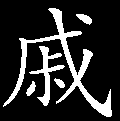
\includegraphics[width=3mm]{../Images/00005}总评:爱众不常,多情不寿;风月情怀,醉人如酒。}

{\href{../Text/part0034_split_000.html\#navto_1_a}{①}``滴'',列本同,杨本、甲辰本作``摘'',蒙、戚本作``拨''。``滴'',江浙方言,两指指尖对掐。}
